\section{Time box 5}
\listoftodos
\subsection{Time box planning}
\begin{figure}[H]
	\begin{centering}
		\missingfigure{Updated timebox figure}
		%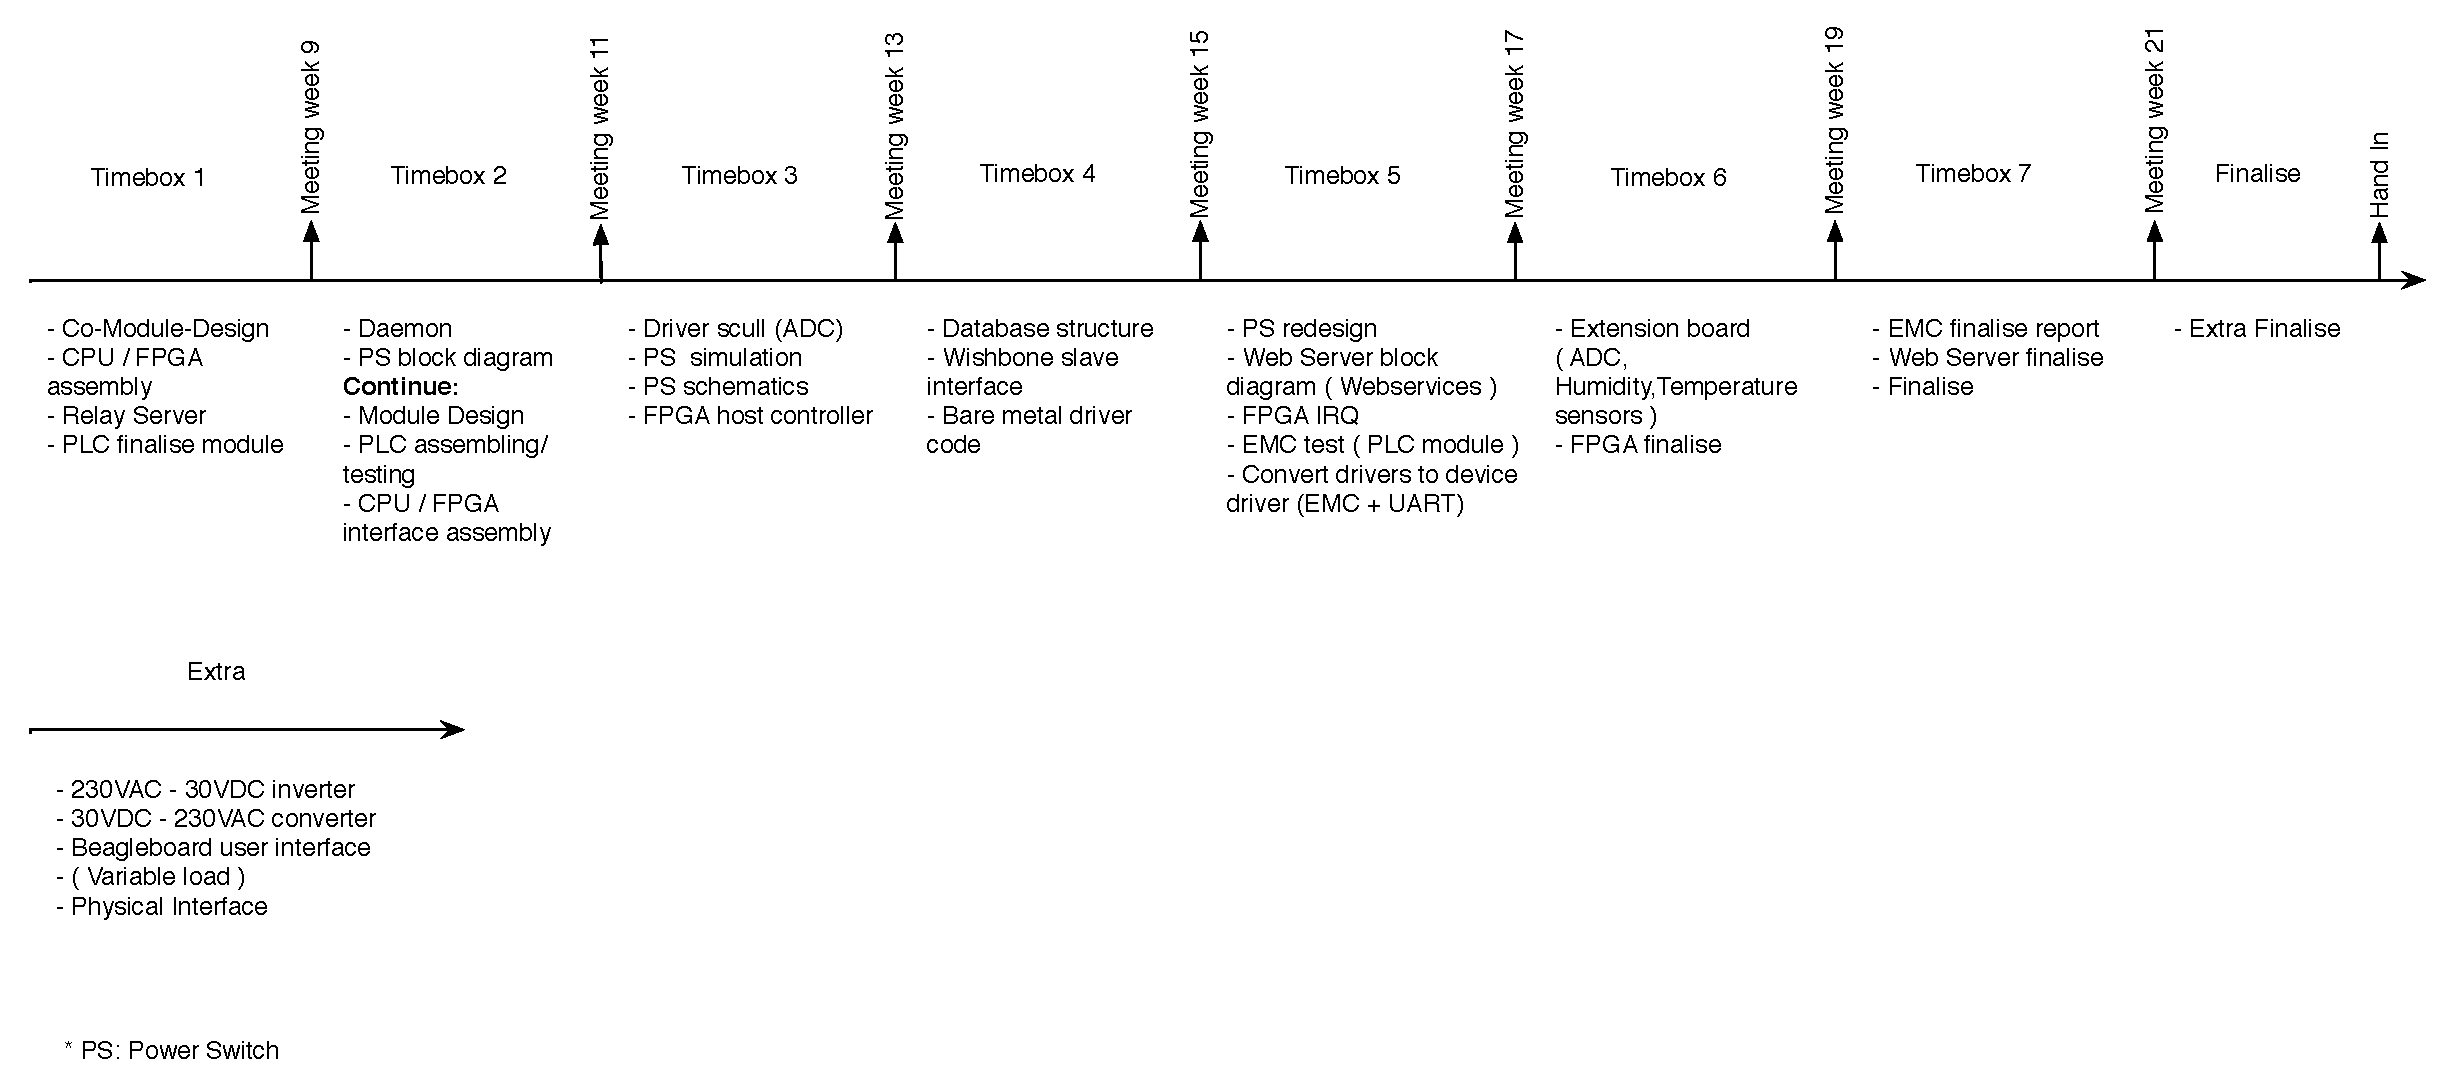
\includegraphics[width=1.0\textwidth]{images/tb_r4.pdf}
		%\caption{Updated time-box}
	\end{centering}
\end{figure}
\subsubsection{Work to be done in this time box}
\begin{itemize}
	\item Something
	\begin{itemize}
		\item some sub something
	\end{itemize}
	\item Some other thing
	\begin{itemize}
		\item some sub thing for other thing
	\end{itemize}
	\item Interrupt register
	\begin{itemize}
		\item Wishbone slave interface
		\item Interrupt signals
		\item Interrupt handling
	\end{itemize}
\end{itemize}
\paragraph{Description:}
\begin{description}
	\item[Something] stuff about something
	\item[Some other thing] about other thing
	\item[Interrupt register] is a block in the Spartan 6, that is allow to interrupt the ARM7 directly. The register is handling other interrupts from the Spartan 6 and tell the ARM7 where the interrupt came from.
\end{description}
\subsubsection{Time planning}
\begin{table}[H]
\centering
	\todo[inline]{Update time}
	\begin{tabular}{|l|c|c|c|c|}
		\hline
		~			& Some thing	& some other thing	& Interrupt Register\\ \hline
		Estimation	& xx			& xx				& 15				\\
		Actual		& xx			& xx				& xx				\\
		Developer	& Dennis		& Paulo				& Theis				\\
		\hline
	\end{tabular}
	\caption{Estimation and actual time used on the project}
\end{table}

\subsection{Something - Dennis}

%			Intro
%					verification specification
%					deployment specification
%
%			Analysis
%
%                Refactored block diagram
%                Refactored class diagram
%                Detailed use cases
%                User interface specification
%                System interface specification
%                Dimensioning specification 
%
%        Design
%
%                UML/SysML deployment view(s)
%                Mechanical specifications and dimensioning
%                HW module specification per block
%                UML SW deployment view
%                Class specification
%                Refactored class diagram
%                Use case scenarios specifications
%                Sequence diagrams
%
%        Implementation
%
%                Mechanical drawings with details explained
%                Electronic diagrams with details explained
%                Source code with details explained
%                Description of integration 
%
%        Verification
%
%                Module tests
%                Integration tests
%                Acceptance test 

\subsection{Some other thing - Jesus}

%			Intro
%					verification specification
%					deployment specification
%
%			Analysis
%
%                Refactored block diagram
%                Refactored class diagram
%                Detailed use cases
%                User interface specification
%                System interface specification
%                Dimensioning specification 
%
%        Design
%
%                UML/SysML deployment view(s)
%                Mechanical specifications and dimensioning
%                HW module specification per block
%                UML SW deployment view
%                Class specification
%                Refactored class diagram
%                Use case scenarios specifications
%                Sequence diagrams
%
%        Implementation
%
%                Mechanical drawings with details explained
%                Electronic diagrams with details explained
%                Source code with details explained
%                Description of integration 
%
%        Verification
%
%                Module tests
%                Integration tests
%                Acceptance test 

\subsection{Interrupt register - Theis}
The interrupt register is made to tune performance by limiting read statements the ARM7 is doing from the Spartan 6. The interrupt register is not by itself fulfilling any requirements, but it is tuning the following: \textit{NF-1.5}\footnote{Requirement is found in table 3.2 in EPRO 3 project energy-hub} and \textit{B-3}\footnote{Requirement is found in table 3.4 in EPRO 3 project energy-hub}
\begin{table}[H]
\centering
	\begin{tabular}{|p{1.2cm}|p{2.3cm}|p{6cm}|p{6cm}|}
	\hline
	ID		& Requirement		& Description																& Comments\\\hline
	NF-1.5	& HW Interface		& 1 start button for the hub. 10 buttons to each start a module.			& It is only reading if the buttons state changes\\\hline
	B-3		& Errors			& Humidity and Temperature sensor will be placed inside the system housing	& The Spartan 6 interrupts if one of the following is happening\\\hline
	B-3.1	& Humidity			& If the humidity is above the maximum level 70\%, the system shuts down	& ARM7 only read on interrupt\\\hline
	B-3.2	& Temperature High	& If the temperature is higher than 55 degrees, the system shuts down		& ARM7 only read on interrupt\\\hline
	B-3.3	& Temperature Low	& If the temperature is below 0 degrees, the system shuts down				& ARM7 only read on interrupt\\\hline
	\end{tabular}
\end{table}
%			Intro
%					verification specification
%					deployment specification
\subsubsection{Analysis}
%			Analysis
%
%                Refactored block diagram
%                Refactored class diagram
%                Detailed use cases
%                User interface specification
%                System interface specification
%                Dimensioning specification 
%
\subsubsection{Design}
%        Design
%
%                UML/SysML deployment view(s)
%                Mechanical specifications and dimensioning
%                HW module specification per block
%                UML SW deployment view
%                Class specification
%                Refactored class diagram
%                Use case scenarios specifications
%                Sequence diagrams
%
\subsubsection{Implementation}
%        Implementation
%
%                Mechanical drawings with details explained
%                Electronic diagrams with details explained
%                Source code with details explained
%                Description of integration 
%
\subsubsection{Verification}
%        Verification
%
%                Module tests
%                Integration tests
%                Acceptance test
\subsubsection{Conclusion}



\subsection{Deployment}
\paragraph{Something}
	%which versions of the prototype the customer will get
	%with what functionality.	
\paragraph{Some other thing}
	%which versions of the prototype the customer will get
	%with what functionality.
\paragraph{Interrupt register}
	%which versions of the prototype the customer will get
	%with what functionality.